%%%%%%%%%%%%%%%%%%%%%%%%
%
%   TIPE Liagre Enzo
%   MPI Faidherbe
%
%%%%%%%%%%%%%%%%%%%%%%%%



\documentclass{beamer}
\usetheme{Berkeley}
\usepackage[french]{babel}
\usepackage[T1]{fontenc}
\usepackage[autolanguage]{numprint}
\usepackage{listings}
\usepackage{array}
\usepackage{xcolor}
\definecolor{commentgreen}{RGB}{2,112,10}
\definecolor{eminence}{RGB}{108,48,130}
\definecolor{weborange}{RGB}{255,165,0}
\definecolor{frenchplum}{RGB}{129,20,83}

\lstset{
    language=C,
    frame=tb,
    tabsize=4,
    showstringspaces=false,
    %upquote=true,
    commentstyle=\color{commentgreen},
    keywordstyle=\color{eminence},
    stringstyle=\color{red},
    basicstyle=\tiny\ttfamily, % basic font setting
    emph={int,char,double,float,unsigned,void,bool},
    emphstyle={\color{blue}},
    escapechar=\&,
    % keyword highlighting
    classoffset=1, % starting new class
    otherkeywords={>,<,.,;,-,!,=,~},
    morekeywords={>,<,.,;,-,!,=,~},
    keywordstyle=\color{weborange},
    classoffset=0,
}

\lstset{
    language=bash,
    frame=tb,
    tabsize=4,
    showstringspaces=false,
    %upquote=true,
    commentstyle=\color{commentgreen},
    keywordstyle=\color{eminence},
    stringstyle=\color{red},
    basicstyle=\tiny\ttfamily, % basic font setting
    emphstyle={\color{blue}},
    escapechar=\&,
    % keyword highlighting
    classoffset=1, % starting new class
    otherkeywords={>,<,.,;,-,!,=,~},
    morekeywords={>,<,.,;,-,!,=,~},
    keywordstyle=\color{weborange},
    classoffset=0,
}

\title{TIPE}
\author{L'émulation et la conservation des logiciels}
\institute{}
\date{\scriptsize LIAGRE Enzo}

\begin{document}
    
    \begin{frame}
        \titlepage\
    \end{frame}

    
    %\begin{frame}{Tables des matières}
    %    \tableofcontents
    %\end{frame}
    
    \section{Présentation du sujet}
    \subsection{Introduction}

    \begin{frame}{Introduction}
        \begin{block}{Émulation}
            L'émulation est le processus par lequel une application reproduit le fonctionnement d'une machine ou d'un autre logiciel.
        \end{block}
        Exemples:
        \begin{itemize}
            \item Un émulateur de terminal
            \item Une machine virtuelle
        \end{itemize}
    \end{frame}

    \begin{frame}{Intérêt}
        \begin{center} 
            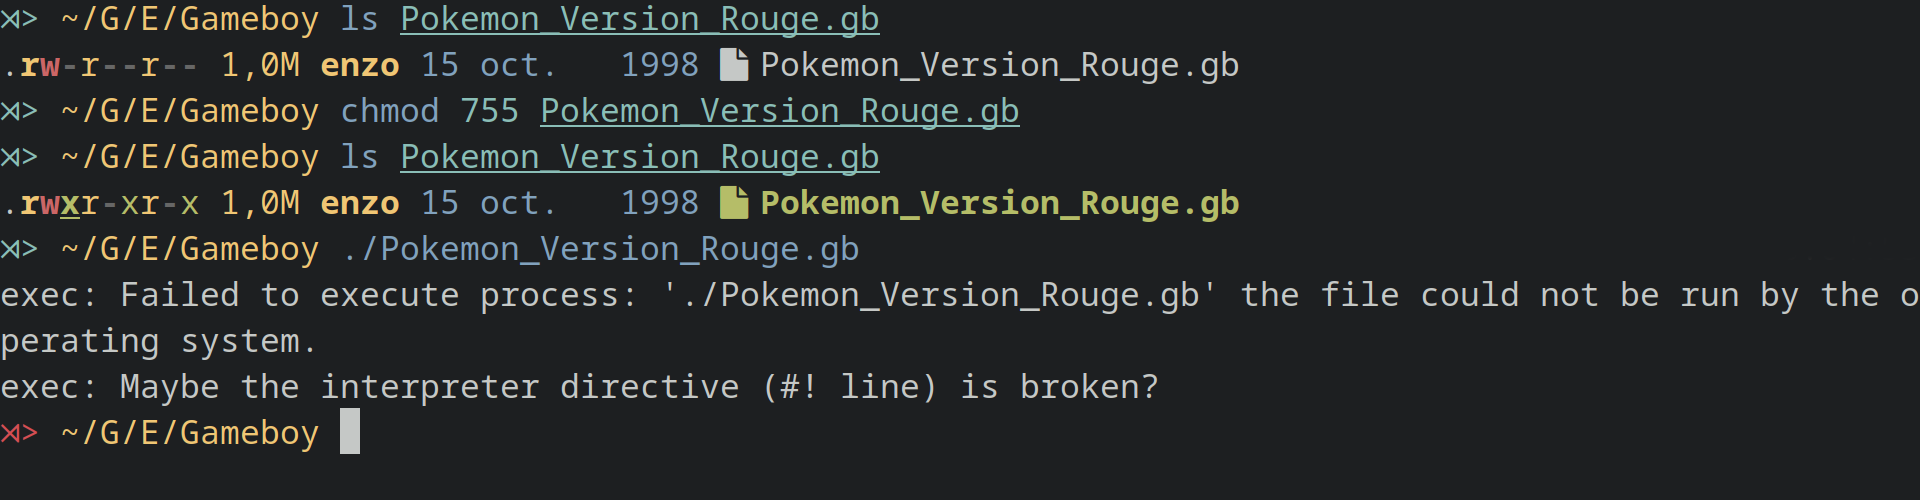
\includegraphics[width=1\textwidth]{images/erreur_permission.png}
        \end{center}   
    \end{frame}

    \begin{frame}{Principe}
        On distingue deux méthodes pour l'émulation.
        \begin{enumerate}
            \item L'émulation de bas niveau (Low-level emulation)
            \begin{itemize}
                \item[\color{white}] $\hookrightarrow$ On reproduit le fonctionnement de la machine en entier.
            \end{itemize}
            \item L'émulation de haut niveau (High-level emulation)
            \begin{itemize}
                \item[\color{white}] $\hookrightarrow$ On reproduit ce que la machine permet.
            \end{itemize}
        \end{enumerate}
        {\color{white} passage de ligne}

        On s'intéressera pour l'instant à l'émulation de bas niveau.
    \end{frame}

    \section{Low-level emulation}
    \subsection{Méthode}
    \begin{frame}{Low-level emulation (LLE)}
        \begin{exampleblock}{Méthode}
            On étudie le sytème afin de savoir comment les composants fonctionnement, puis on les implémentes.
        \end{exampleblock}
        $\hookrightarrow$ On implémente des machines entières donc on privilégie un language de bas niveau.
    \end{frame}

    \subsection{Exemple: La GameBoy}
    \begin{frame}{L'émulation d'un jeu GameBoy}
        \begin{center}
            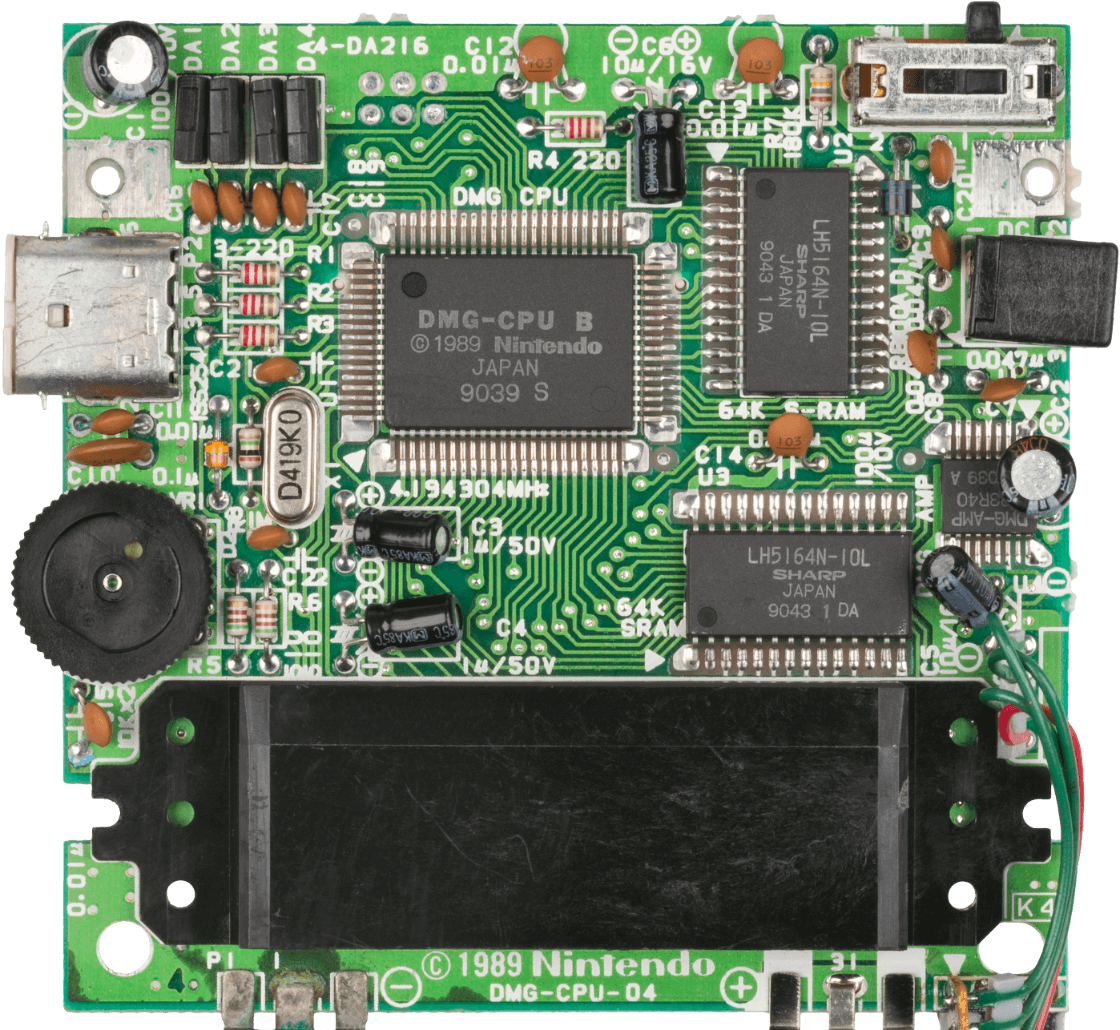
\includegraphics[width=0.7\textwidth]{images/carte_mere.png}
        \end{center}
    \end{frame}

    \begin{frame}{L'émulation d'un jeu GameBoy}
        \begin{center}
            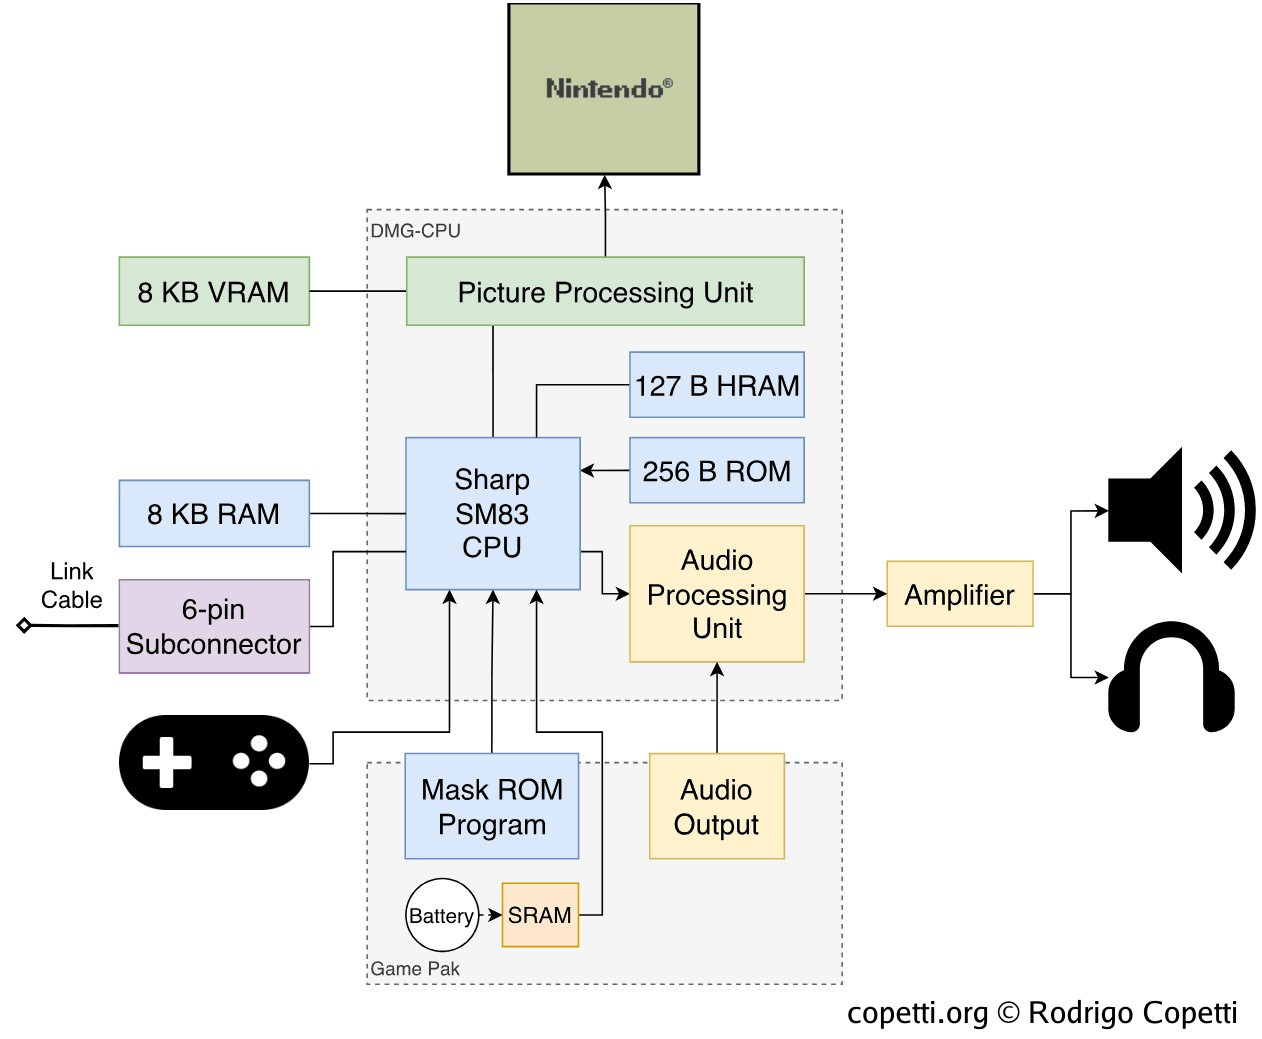
\includegraphics[width=0.8\textwidth]{images/diagrame.png}
        \end{center}
    \end{frame}

    \subsection{Implémentation}
    \begin{frame}{La Structure}
        On suppose que la GameBoy n'est composée que
        \begin{itemize}
            \item d'un lecteur cartouche
            \item d'un CPU
        \end{itemize}

        {\color{white} passage de ligne}

        On représente le lecteur cartouche par un tableau $8 \times 16^3$ entiers naturels codés sur $8-$bits.
    \end{frame}

    \begin{frame}{Le CPU}
        Le processeur de la GameBoy est un Sharp SM83.\\
        Celui-ci est $8-$bit. Autrement dit ses régistre sont de taille $1$ octet.
        
        {\color{white} passage de ligne}

        \begin{block}{Registre}
            Un registre est un bloc de la mémoire interne du processeur.
            Il s'agit de la mémoire la plus rapide d'un ordinateur.
        \end{block}
        C'est dans ces bloc que le processeur effectue ses calcules.
    \end{frame}

    \begin{frame}{L'organisation}
        Le Sharp SM83 contient 10 registres.
        \begin{columns}
            \begin{column}{0.5\textwidth}
                \begin{center}
                    \begin{tabular}{ | m{1.5cm} | m{1.5cm} | } 
                        \hline
                        A & F \\ 
                        \hline
                        B & C \\ 
                        \hline
                        D & E \\ 
                        \hline
                        H & L \\
                        \hline
                    \end{tabular}
                \end{center}
            \end{column}
            \begin{column}{0.5\textwidth}
                \begin{center}
                    \begin{tabular}{ | m{1.5cm} | }
                        \hline
                        SP \\ 
                        \hline
                        PC \\ 
                        \hline
                    \end{tabular}
                \end{center}
            \end{column}
        \end{columns}
    \end{frame}

    \begin{frame}{L'organisation}
        Le Sharp SM83 contient 10 registres.
        \begin{columns}
            \begin{column}{0.5\textwidth}
                \renewcommand{\arraystretch}{2} 
                \begin{tabular}{ m{0.1cm} | m{1.4cm} | m{1.4cm} | m{0.1cm} } 
                    \cline{2-3}
                    A
                    &$0 \rightarrow 255$
                    &$0 \rightarrow 255$
                    & F \\
                    \cline{2-3}
                    B
                    &$0 \rightarrow 255$
                    &$0 \rightarrow 255$
                    & F \\
                    \cline{2-3}
                    C
                    &$0 \rightarrow 255$
                    &$0 \rightarrow 255$
                    & F \\ 
                    \cline{2-3}
                    D
                    &$0 \rightarrow 255$
                    &$0 \rightarrow 255$
                    & E \\
                    \cline{2-3}
                \end{tabular}
            \end{column}
            \begin{column}{0.4\textwidth}
                \begin{center}
                    \renewcommand{\arraystretch}{1.2} 
                    \begin{tabular}{| m{1.8cm} |}
                        \multicolumn{1}{m{1.8cm}}{SP}\\ 
                        \hline
                        $0 \rightarrow 65535$\\
                        \hline
                        $0 \rightarrow 65535$\\
                        \hline
                        \multicolumn{1}{m{1.8cm}}{PC}\\ 
                    \end{tabular}
                \end{center}
            \end{column}
        \end{columns}
    \end{frame}

    \subsection{Exécution}
    \begin{frame}{Exécution}
        Si le CPU n'est qu'une structure avec ses registres représentés en variables, on a
        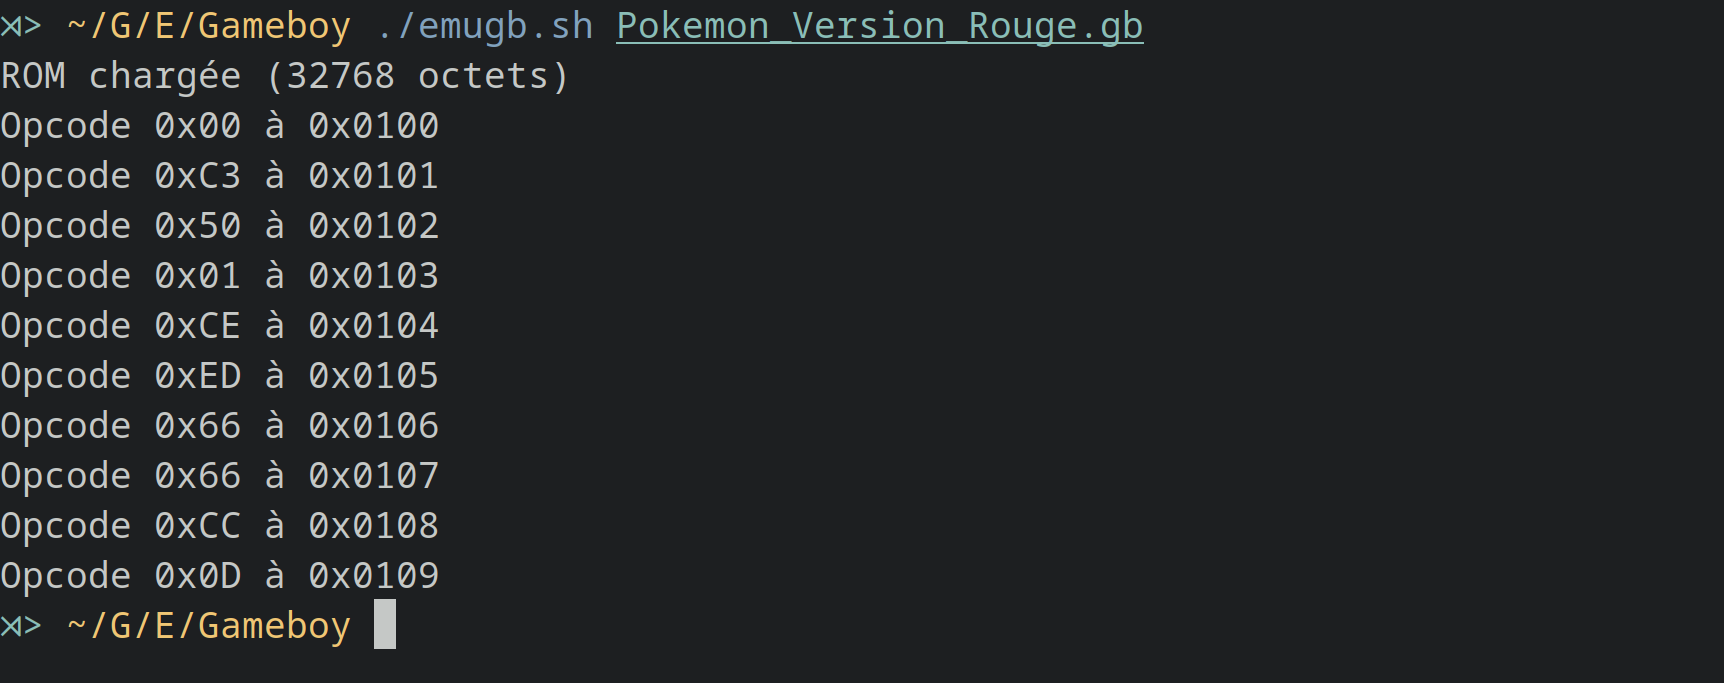
\includegraphics[width=1\textwidth]{images/execution.png}
    \end{frame}

    \section{Conclusion}
    \begin{frame}{Conclusion}
        En suivant la même méthode, on peut, en théorie, émuler n'importe quel logiciel.

        {\color{white} passage de ligne}

        Cependant, reproduire la machine en entier pose des problèmes de performance.
    \end{frame}

    \begin{frame}{En prolongement}
        La suite du TIPE se portera sur l'émulation de haut niveau.

        {\color{white} passage de ligne}

        On pourrait envisager
        \begin{itemize}
            \item implementer l'émulateur en entier
            \item effectuer des test de performances entre LLE / HLE
        \end{itemize}
    \end{frame}

    \begin{frame}{Du négatif}
        Il rest important de remarquer que
        \begin{itemize}
            \item Ce TIPE est très empirique
            \item L'émulation ne serait utile si tous les sytèmes avait un même systeme d'exploitation
            \item Il est légalement difficile de travailler sur ce sujet
        \end{itemize}
    \end{frame}

    \appendix
    \section{Références}
    \begin{frame}{Bibliographie}
        \begin{enumerate}
            \item \guillemotleft\ Stack processor architecture and development methods suitable for dependable
applications.\ \guillemotright\ Mehdi Jallouli, Camille Diou, Fabrice Monteiro, Abbas Dandache.
            \item \guillemotleft\ Game Boy: Complete Technical Reference \guillemotright\ {\color{blue}\underline{\url{https://gekkio.fi}}}, Révision 164.
            \item L'article \guillemotleft\ Game Boy / Color Architecture $-$ A Practical Analysis \guillemotright\ écrit par Rodrigo Copetti {\color{blue} \underline{\href{https://www.copetti.org/writings/consoles/game-boy/}{www.copetti.org/writings/consoles/game-boy/}}}.
            \item La série \guillemotleft\ The Game Boy, a hardware autopsy \guillemotright\ par JackTech {\color{blue} \underline{\url{https://www.youtube.com/@jacktech5101}}}.
        \end{enumerate}
    \end{frame}

    \begin{frame}{Ressources}
        \begin{enumerate}
            \item Architecture du processeur \guillemotleft\ Sharp SM83 \guillemotright\ {\color{blue} \underline{\url{https://gbdev.io/gb-opcodes//optables/}}}.
            \item Fichier ROM d'une cartouche de \textit{Pokémon Version Rouge} développé par Game Freak.
            \item Quelques illustrations de \guillemotleft\ Game Boy / Color Architecture $-$ A Practical Analysis \guillemotright\ écrit par Rodrigo Copetti {\color{blue} \underline{\href{https://www.copetti.org/writings/consoles/game-boy/}{www.copetti.org/writings/consoles/game-boy/}}}.
        \end{enumerate}
    \end{frame}

    \section{Code}
    \begin{frame}{emugb.sh}
        \lstset{language=bash}
        \lstinputlisting[breaklines]{code/emugb.sh}
    \end{frame}

    \begin{frame}[allowframebreaks]{CPU.h}
        \lstset{language=C}
        \lstinputlisting[breaklines]{code/CPU.h}
    \end{frame}

    \begin{frame}[allowframebreaks]{CPU.c}
        \lstinputlisting[breaklines]{code/CPU.c}
    \end{frame}

    \begin{frame}[allowframebreaks]{SoC.h}
        \lstinputlisting[breaklines]{code/SoC.h}
    \end{frame}

    \begin{frame}[allowframebreaks]{Gameboy.h}
        \lstinputlisting[breaklines]{code/Gameboy.h}
    \end{frame}

    \begin{frame}[allowframebreaks]{Gameboy.c}
        \lstinputlisting[breaklines]{code/Gameboy.c}
    \end{frame}

    \begin{frame}[allowframebreaks]{emu.c}
        \lstinputlisting[breaklines]{code/emu.c}
    \end{frame}
    
\end{document}
